

\documentclass[journal, twoside]{IEEEtran}
% *** CITATION PACKAGES ***
%

%\usepackage[brazilian]{babel}%%%%% for papers in portuguese
%\usepackage[spanish]{babel}%%%%% for papers in Spanish
\usepackage{fancyhdr} %used for header
\pagestyle{fancy} %also used for header
\usepackage{lipsum}
\usepackage[utf8]{inputenc}
\usepackage[T1]{fontenc}

\usepackage{graphicx} %% for loading jpg figures
\usepackage{subfig}
\usepackage{nccmath}
\usepackage{color}
\usepackage{cite}
\usepackage{acro}
\usepackage{float}
\usepackage{scalerel}
\usepackage{tikz}
\usetikzlibrary{svg.path}

\definecolor{orcidlogocol}{HTML}{A6CE39}
\tikzset{
  orcidlogo/.pic={
    \fill[orcidlogocol] svg{M256,128c0,70.7-57.3,128-128,128C57.3,256,0,198.7,0,128C0,57.3,57.3,0,128,0C198.7,0,256,57.3,256,128z};
    \fill[white] svg{M86.3,186.2H70.9V79.1h15.4v48.4V186.2z}
                 svg{M108.9,79.1h41.6c39.6,0,57,28.3,57,53.6c0,27.5-21.5,53.6-56.8,53.6h-41.8V79.1z M124.3,172.4h24.5c34.9,0,42.9-26.5,42.9-39.7c0-21.5-13.7-39.7-43.7-39.7h-23.7V172.4z}
                 svg{M88.7,56.8c0,5.5-4.5,10.1-10.1,10.1c-5.6,0-10.1-4.6-10.1-10.1c0-5.6,4.5-10.1,10.1-10.1C84.2,46.7,88.7,51.3,88.7,56.8z};
  }
}

\newcommand\orcidicon[1]{\href{https://orcid.org/#1}{\mbox{\scalerel*{

\begin{tikzpicture}[yscale=-1,transform shape]
\pic{orcidlogo};
\end{tikzpicture}
}{|}}}}

\renewcommand{\headrulewidth}{0pt}% disable the underline of the header part

% *** GRAPHICS RELATED PACKAGES ***
%
\ifCLASSINFOpdf
  % \usepackage[pdftex]{graphicx}
  % declare the path(s) where your graphic files are
  % \graphicspath{{../pdf/}{../jpeg/}}
  % and their extensions so you won't have to specify these with
  % every instance of \includegraphics
  % \DeclareGraphicsExtensions{.pdf,.jpeg,.png}
\else
  % or other class option (dvipsone, dvipdf, if not using dvips). graphicx
  % will default to the driver specified in the system graphics.cfg if no
  % driver is specified.
  % \usepackage[dvips]{graphicx}
  % declare the path(s) where your graphic files are
  % \graphicspath{{../eps/}}
  % and their extensions so you won't have to specify these with
  % every instance of \includegraphics
  % \DeclareGraphicsExtensions{.eps}
\fi
% graphicx was written by David Carlisle and Sebastian Rahtz. It is
% required if you want graphics, photos, etc. graphicx.sty is already
% installed on most LaTeX systems. The latest version and documentation
% can be obtained at: 
% http://www.ctan.org/pkg/graphicx
% Another good source of documentation is "Using Imported Graphics in
% LaTeX2e" by Keith Reckdahl which can be found at:
% http://www.ctan.org/pkg/epslatex
%
% latex, and pdflatex in dvi mode, support graphics in encapsulated
% postscript (.eps) format. pdflatex in pdf mode supports graphics
% in .pdf, .jpeg, .png and .mps (metapost) formats. Users should ensure
% that all non-photo figures use a vector format (.eps, .pdf, .mps) and
% not a bitmapped formats (.jpeg, .png). The IEEE frowns on bitmapped formats
% which can result in "jaggedy"/blurry rendering of lines and letters as
% well as large increases in file sizes.
%
% You can find documentation about the pdfTeX application at:
% http://www.tug.org/applications/pdftex

\usepackage{hyperref} %<--- Load after everything else
\begin{document}
 
\setcounter{page}{1}%%%% HERE SET THE PAGE NUMBER
\title{Análise de previsão de desvio para as \\ nove variações do algoritmo de dois níveis}


\author{Universidade Estadual de Maringá\\
Ciência da Computação - Departamento de Informática\\ 
Diogo Alves de Almeida \\
Email: ra95108@uem.br \\
09 de dezembro de 2021}

\markboth{9 de Dezembro de 2021}{Diogo Alves de Almeida}  

\maketitle

\begin{abstract}
Com a evolução da tecnologia e dos processadores superescalares, que conseguem explorar o paralelismo a nível de instrução, surgiu-se a técnica de previsão de desvio para tentar antecipar o resultado de desvios condicionais a fim de ter um fluxo ininterrupto e trazer um melhor desempenho para o processador. Esse trabalho tem como objetivo analisar as implementações das nove variações de previsão de desvio dinâmica para dois níveis e verificar qual a melhor estratégia para os programas de testes escolhido e mostrar que a variação \textit{SAg} tem um desempenho de previsão enquanto \textit{Gag} consegue ser superior em relação ao tempo de execução.
\end{abstract}
.
\begin{IEEEkeywords}
Arquitetura de computadores, previsor de desvio, algoritmo de dois níveis.
\end{IEEEkeywords}

\IEEEpeerreviewmaketitle

\section{Introdução}
O paralelismo de serviços é um dos temas mais abordados quando falamos de processadores e sua melhora de desempenho. A técnica mais utilizada para aumentar esse desempenho é o \textit{pipeline}, que consiste em aproveitar a maior parte possível do processador que não esteja sendo utilizada. De modo geral, é uma técnica que permite que a realização da busca de uma ou mais instruções além da próxima a ser executada, logo, assim que uma instrução termina o primeiro estágio e parte para o segundo, a próxima instrução já ocupa o primeiro estágio. Porém, o paralelismo em arquiteturas superescalares é limitado pois além das dependências de controle, provocadas pelos desvios, também temos as dependências verdadeiras (também conhecidas como dependências de dados), para resolver essas dependências é usada a previsão de desvio.

O previsor de desvio é um componente essencial nos processadores modernos, uma vez que sua alta precisão pode melhorar desempenho e reduzir a energia, diminuindo o número de instruções executadas no caminho incorreto. Porém, reduzir a latência e a sobrecarga de armazenamento do previsor enquanto mantém a alta precisão apresenta desafios significativos \cite{mitall}.

Atualmente há várias maneiras de implementar um previsor de desvio e essas decisões impactam significativamente no desempenho do processador, portanto esse trabalho tem como objetivo analisar as implementações de previsão de desvio dinâmica para dois níveis e verificar qual a melhor estratégia para os programas de testes escolhidos.

Na seção \ref{previsao} temos os fundamentos sobre previsão de desvios e os algoritmos implementados, na seção \ref{metodologia} temos o detalhamento de como o algoritmo foi implementado e como foi avaliado. Por fim, na seção \ref{analise}, temos os resultados encontrados com as simulações.


\section{Previsão de desvio} \label{previsao}
Segundo \cite{pizzol}, o desempenho do pipeline só será máximo se não ocorrer bloqueio da execução contínua dos diversos estágios de execução. As instruções de desvio provocam uma queda do desempenho dos processadores uma vez que bloqueiam a operação contínua do pipeline por não ser sempre possível conhecer o resultado do comando de desvio (tomado ou não tomado) durante o estágio de busca.

Os desvios e as trocas de fluxos são classificadas em quatro tipos:
\begin{itemize}
    \item Desvios condicionais
    \item Desvios incondicionais
    \item Chamadas de procedimentos
    \item Retorno de procedimentos
\end{itemize}

Para trazer um desempenho melhor do pipeline temos a previsão de desvio que ajuda resolver os perigos de saltos que assume um dado destino para o salto e continua a execução a partir do destino, ao invés de esperar verificar o destino atual. Com a previsão de desvio é possível ter um aumento do número de instruções disponíveis para o despacho e aumento de paralelismo de instrução permitindo que o trabalho útil seja concluído enquanto se espera pela resolução do desvio. Por exemplo, experimentos em processadores reais mostraram que reduzir as previsões erradas de ramos pela metade melhorou o desempenho do processador em 13\%	 \cite{mitall}.

\subsection{Estratégias de previsão de desvio}
As estratégias de previsão de desvio podem ser divididas em duas categorias básicas:
\begin{itemize}
    \item Desvio estático
    \item Desvio dinâmico
\end{itemize}

A previsão estática para um desvio será sempre o mesmo e pode ser realizado no nível de software, pelo compilador, ou no nível de hardware, em tempo de execução. Essa estratégia é implementada a partir de quatro variações: assumir que todos os saltos serão tomados, assumir que todos os saltos não serão tomados, assumir que todos os desvios para um determinado \textit{operation code} serão tomados ou assumir que os saltos para trás serão tomados e os que os saltos para frente serão não tomados \textit{(BTFN - backward-taken, forward not-taken)}.

 A previsão dinâmica, usualmente mais eficientes que as estáticas, armazenam informações coletadas das instruções em tempo de execução e quando um desvio for novamente executado, o previsor verifica o que ocorreu anteriormente e decide, baseado nessa informação, o resultado dessa nova operação.

Dentro da previsão dinâmica temos duas estratégias: utilizar 1 bit e utilizar 2 bits. A estratégia de 1 bit é mais simples, enquanto a de 2 bits é mais robusta e eficiente. Para esse trabalho iremos utilizar a estratégia de dois bits que contém uma máquina de estados (histórico ou contador saturado) que define se o salto será ou não tomado na próxima execução. Na figura \ref{contador_saturado} temos o autômato utilizado para a previsão com 2 bits.

\begin{figure}[H]
    \centering
    \captionsetup{justification=centering}
    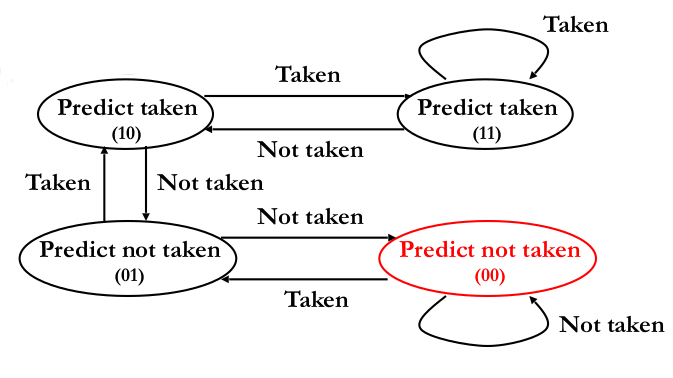
\includegraphics[width=2.5in]{figure/contador_saturado.jpeg}
    \caption{Autômato de 2 bits (contador saturado).}
    \label{contador_saturado}
\end{figure}

Como podemos ver na figura, os estados com bits iguais (TT e NN), a previsão segue o resultado atual enquanto quando os bits são diferentes ocorre uma alteração de previsão seguindo o estado mais antigo como decisão. Com essa estratégia de 2 bits é possível alcançar uma taxa média de acerto individual de 90\% \cite{lee_smith}. 

Usando 2 bits em vez de 1, um desvio que favoreça bastante a situação “tomado” ou “não tomado”, como muitos desvios fazem, será previsto incorretamente apenas uma vez. Os 2 bits são usados para codificar os quatro estados no sistema. O esquema de 2 bits é um caso geral de uma previsão baseada em contador, incrementado quando a previsão é exata e decrementado em caso contrário, e
utiliza o ponto intermediário desse intervalo como divisão entre desvio tomado e não tomado \cite{patterson_hennessy}. 

Par a previsão de desvio dinâmica de dois níveis tempos que o primeiro nível armazena o histórico dos \textit{k} últimos desvios, enquanto que o segundo nível armazena o que aconteceu com as últimas \textit{j} ocorrências de um padrão específico dos \textit{k} desvio. O primeiro nível é denominadamente chamado de \textit{Branch History Register} (BHR), o segundo nível é denominado \textit{Pattern History Table} (PHT), enquanto um conjunto de BHRs é chamado de \textit{Branch History Table} (BHT).

O endereço do salto é mapeado para o acesso no primeiro nível (BHR), o valor obtido em BHR significa o endereço para acessar o segundo nível (PHT) que contém o valor de 2 bits que será definido a previsão do salto atual como vimos na figura \ref{contador_saturado} anteriormente. A tabela do segundo nível deve conter uma entrada de cada histórico possível em primeiro nível, logo, temos que PHT deve ter o tamanho de \(2^k\) (possibilidades).

Os dois níveis podem ter 3 classificações diferentes de acordo com a sua implementação e estratégia:

\begin{itemize}
    \item G/g: para o primeiro nível (G) é guardado o histórico dos últimos \textit{k} desvios encontrados, assim, apenas um BHR é produzido. Para o segundo nível (g) é definido como os padrões serão associados sendo os \textit{k} últimos desvios encontrados, criando também apenas um PHT. 
    \item P/p: para o primeiro nível (P) é guardado o histórico das últimas \textit{k} ocorrências de um mesmo desvio, sendo assim, existirá um BHR para cada instrução de desvio. Para o segundo nível (p) é definido como os padrões serão associados sendo as \textit{k} últimas ocorrências de um mesmo desvio.
    \item S/s: para o primeiro nível (S) é guardado o histórico das últimas \textit{k} ocorrências de um mesmo conjunto de desvios, sendo assim, cada BHR está associado a um conjunto de desvios. Para o segundo nível (s) é definido como os padrões serão associados sendo as \textit{k} últimas ocorrências de um conjunto de desvios. 
\end{itemize}

Portanto, com essa variações surgiu nove diferentes variações de previsores de dois níveis como podemos ver na figura \ref{esquema_2_niveis} a seguir.

\begin{figure}[H]
    \centering
    \captionsetup{justification=centering}
    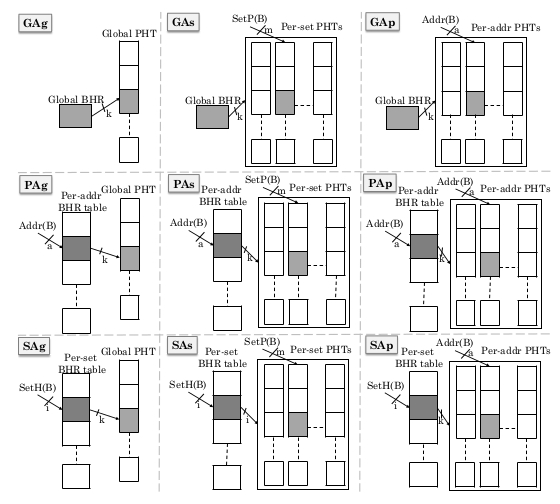
\includegraphics[width=3.4in]{figure/esquemas_dois_niveis.jpeg}
    \caption{Variações de previsores de dois níveis.}
    \label{esquema_2_niveis}
\end{figure}

\section{Metodologia} \label{metodologia}
A ferramenta que foi utilizado para análise dos algoritmos é a ferramenta PIN que consistem em uma estrutura de instrumentação binária dinâmica para as arquiteturas de conjunto de instruções \textit{IA-32}, \textit{x86-64} e \textit{MIC} que permite a criação de ferramentas dinâmicas de análise de programa. \cite{levi}

Para o desenvolvimento do trabalho foi disponibilizado no \textit{moodle} da disciplina um repositório com um exemplo de código de análise de previsão de desvio para ser utilizado com a ferramenta PIN. O programa presente no repositório continha um algoritmo que analisava através da ferramenta PIN os saltos do programa que estava sendo executado e no fim da execução trazia diversas estatísticas importantes para o desenvolvimento do trabalho para que pudéssemos realizar a comparação dos algoritmos.

As variações foram implementadas em um único arquivo chamado \textit{bp\_custom.cpp} no qual havia 3 funções principais que foram onde o desenvolvimento foi realizado. Na primeira função chamada \textit{init} foi implementado a inicialização das estruturas de dados utilizadas, mais precisamente a(s) lista(s) de BHR(s) e PHT(s), durante a execução do programa para a previsão do desvio. Na segunda função chamada \textit{predict} foi implementado a tomada de decisão de salto definindo se seria tomado ou não tomado, essa função recebia um objeto no qual havia um atributo que era definido como a posição da instrução (\textit{program counter}) do salto no qual em algumas variações é utilizado para obter a posição correta do BHR e PHT.  Na terceira função chamada \textit{update} foi implementado a verificação se o salto atual foi tomado ou não e atualização das tabelas necessárias, essa função recebia um objeto como parâmetro que continha os atributos \textit{taken}, que definia se o salto foi ou não tomado, como também a posição de instrução do salto. Vale ressaltar que os objetos recebidos como parâmetros havia vários atributos que não foram utilizados na implementação.

Para trabalhar com os bits foi utilizado o \textit{bitset} da biblioteca padrão do C++, como o \textit{bitset} permite ser criado com tamanho variável para as tabelas BHRs cada elemento era um \textit{bitset} de tamanho \textit{k} enquanto que para as tabelas PTHs cada elemento era um \textit{bitset} de tamanho 2 representando o estado atual do autômato de 2 bits. Na função \textit{update}, após ser verificado se o salto foi ou não tomado as tabelas eram atualizadas onde o elemento correto de BHR e PHT era alterado realizando um \textit{shift} no bit menos significativo com a representação do salto atual (1 para salto tomado e 0 para não tomado), assim era atualizado o histórico dos \textit{k} últimos saltos como também o estado atual do autômato.

As tabelas utilizadas em todas as funções são variáveis globais criadas especificamente para cada variação. Além das variáveis das tabelas temos também as variáveis de definição do tamanho do bit (k), bit mais significativo para ser utilizado para acessar um elemento de PHT (m), bit menos significativo para ser utilizado para acessar um elemento de PHT (a), bit mais significativo para ser utilizado em BHR nas variações SA (i), como também uma variável \textit{string} que define qual variação será utilizado no momento da execução (b). Podemos ver na tabela \ref{tab:params} a seguir as variáveis \textit{int} dita anteriormente com os valores definidos para teste.

\begin{table}[H]
\centering
\begin{tabular}{|c|c|}
\hline
\textbf{Variável} & \textbf{Valor utilizado} \\ \hline
k                   & 12                       \\ \hline
i                   & 4                        \\ \hline
m                   & 4                        \\ \hline
a                   & 8                        \\ \hline
\end{tabular}
\caption{Variáveis globais e valores utilizados}
\label{tab:params}
\end{table}

Para a execução dos testes foi implementado scripts utilizando o interpretador \textit{GNU Bash} no qual para cada variação era alterado a linha 24 do arquivo \textit{bp\_custom.cpp} definindo qual variação seria executada no momento, em seguida foi compilado o arquivo e executado o programa \textit{heat-3d} na coleção de \textit{benchmarks} do \textit{PolyBench/C} \cite{polybench}. O programa \textit{heat-3d} foi compilado com entrada de tamanho \textit{large} para termos uma precisão maior dos resultados. Também foi realizado testes com o programa \textit{AStar} que estava contido no repositório disponibilizado para a realização de trabalho, para esse programa foi utilizado a entrada \textit{big} para melhor precisão dos resultados.


\section{Análise e Discussão} \label{analise}
Após executado todas as variação foi estudado as estatísticas geradas e também analisado o tempo de execução dos programas. Os valores para a geração dos gráficos foram calculados tendo como base a variação \textit{SAg} e calculados a porcentagem em relação a ela. A escolha do \textit{SAg} foi devido a percepção dos resultados que aparentavam ter sido o melhor algoritmo. 

Para encontrar o melhor algoritmo foi obtido dos arquivos de saída as variáveis \textit{Taken Branches}, \textit{Taken Predicted}, \textit{Not Taken Branches} e \textit{Not Taken Predicted} no qual informavam a quantidade de saltos realmente tomados pelo processador e a quantidade de saltos que foi previsto. Foi escolhido essas variáveis pois a porcentagem de precisão da variável \textit{Overall Hits} continha apenas 4 casas decimais não trazendo uma precisão desejada nos gráficos uma vez que os valores estavam bem parecidos. A seguir temos os gráficos com o comparativo de todas as variações para os 2 programas executados. 
\begin{figure}[H]
    \centering
    \captionsetup{justification=centering}
    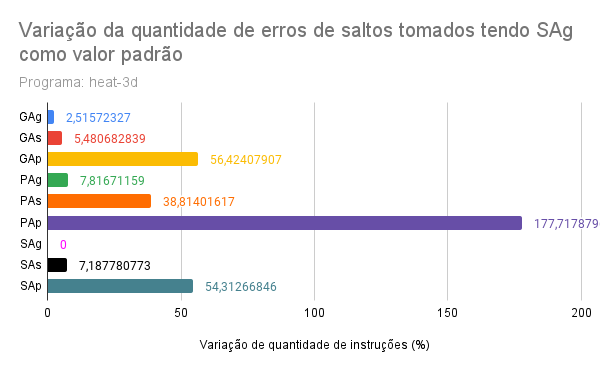
\includegraphics[width=3.4in]{figure/saltos_tomados_(heat-3d).png}
    \caption{Variação da quantidade de erros de saltos tomados tendo SAg como valor padrão (\textit{heat-3d}).}
    \label{fig:saltos-nao-tomados-heat}
\end{figure}

\begin{figure}[H]
    \centering
    \captionsetup{justification=centering}
    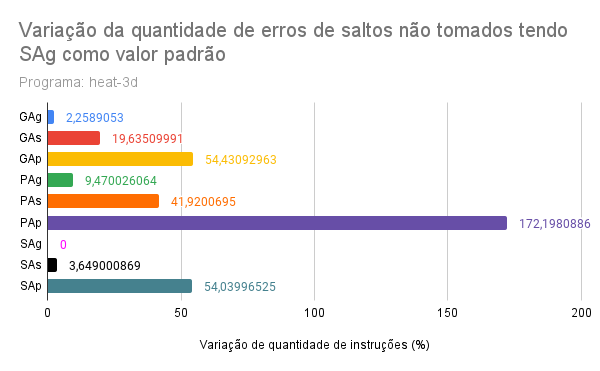
\includegraphics[width=3.4in]{figure/saltos_nao_tomados_(heat-3d).png}
    \caption{Variação da quantidade de erros de saltos não tomados tendo SAg como valor padrão (\textit{heat-3d}).}
    \label{fig:saltos-nao-tomados-heat}
\end{figure}

\begin{figure}[H]
    \centering
    \captionsetup{justification=centering}
    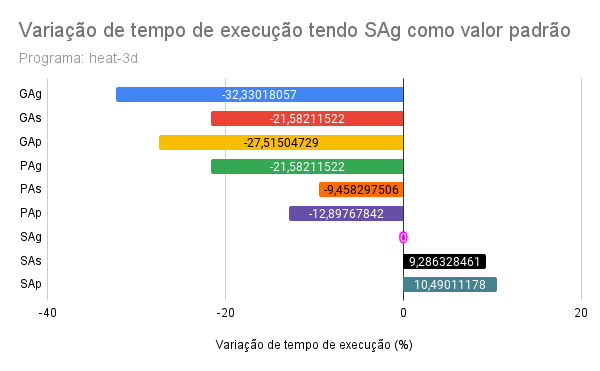
\includegraphics[width=3.4in]{figure/tempo_de_exec_(heat-3d).png}
    \caption{Tempo de execução execução do programa (\textit{heat-3d}).}
    \label{fig:tempo-heat}
\end{figure}

\begin{figure}[H]
    \centering
    \captionsetup{justification=centering}
    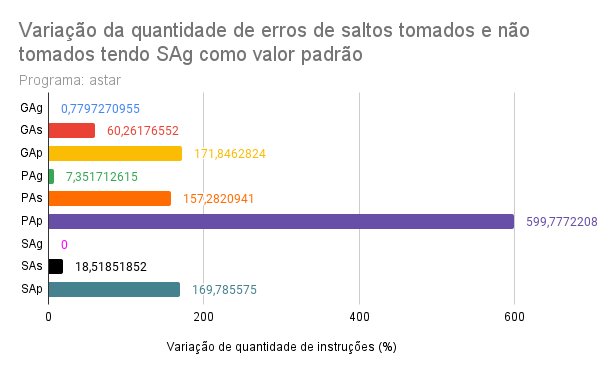
\includegraphics[width=3.4in]{figure/saltos_(astar).png}
    \caption{Variação da quantidade de erros de saltos tomados e não tomados tendo SAg como valor padrão (\textit{astar}).}
    \label{fig:saltos}
\end{figure}

\begin{figure}[H]
    \centering
    \captionsetup{justification=centering}
    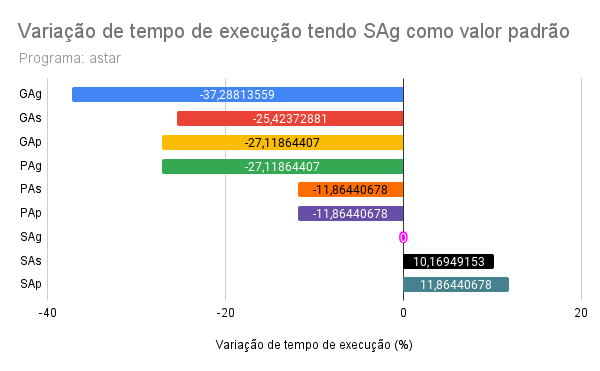
\includegraphics[width=3.4in]{figure/tempo_de_exec_(astar).png}
    \caption{Tempo de execução execução do programa (\textit{astar}).}
    \label{fig:tempo-astar}
\end{figure}

Ao calcular a variação de saltos tomados e não tomados, foi analisado que para o programa \textit{astar} os algoritmos teve os mesmo valores de variação percebendo um padrão no comportamento dos algoritmos, o que não pode ser visto no programa \textit{heat-3d}. Portanto, o gráfico da figura \ref{fig:saltos} é uma representação geral do comportamento do programa \textit{astar} sendo eles para previsão de saltos tomados e não tomados.

A partir dos gráficos podemos verificar que para o programa \textit{heat-3d} as variações \textit{GAg}, \textit{GAs}, \textit{PAg} e \textit{SAg} tiveram um desempenho próximo em relação aos erros de saltos tomados e não tomados tendo o \textit{SAg} o melhor resultado, porém, quando comparado o tempo de execução pode-se perceber uma diferença significativa mostrando que o \textit{GAg} foi 32,3301\% mais rápido, sendo assim, o tempo de execução foi um fator muito importante para concluir que o \textit{GAg} acaba sendo o melhor algoritmo para o programa.

Por outro lado, podemos verificar que o pior algoritmo foi da variação \textit{PAp} que teve um desempenho muito fraco comparado as outras variações enquanto seu tempo de execução não teve nenhuma relevância sendo o quarto mais lento.

Para o programa \textit{astar} foi verificado que o melhor algoritmo para previsão dos desvios foi o \textit{SAg}, tendo \textit{GAg}, \textit{PAg}, \textit{SAs} muito próximos em relação ao desempenho de previsão. Porém, assim como no programa \textit{heat-3d}, o tempo de execução foi o fator determinante para concluir que o \textit{GAg} foi 37,2881\% mais rápido. Podemos verificar também que o pior algoritmo para o programa em questão também acabou sendo o \textit{PAp}.

\section{Conclusões} \label{conclusao}

Com isso, pode-se concluir que quando analisado apenas o desempenho do algoritmo em relação a previsão de desvios a variação \textit{SAg} acaba sendo a melhor para os programas em questão. Porém, quando adicionamos a variável de tempo de execução para analisar os algoritmos, o programa \textit{GAg} acaba sendo a melhor opção tendo uma superioridade significativa.

\bibliographystyle{ieeetr}  

\ifCLASSOPTIONcaptionsoff
  \newpage
\fi

\begin{thebibliography}{1}

\bibitem{mitall}
S. MITTAL. \emph{A Survey of Techniques for Dynamic Branch Prediction}, 2018.

\bibitem{patterson_hennessy}
D. A. PATTERSON, J. L. HENNESSY, \emph{Computer Organization and Design}, 5th ed. Boston, EUA: Morgan Kaufmann (an imprint of Elsevier), 2018. 

\bibitem{pizzol}
G. D. PIZZOL, \emph{Previsão de Desvios em Arquiteturas Multitarefas Simultâneas}, Dissertação de mestrado, Universidade Federal do Rio Grande do Sul. Programa de Pós-Graduação em Computação, Porto Alegre, RS, 2005, Seção 2.

\bibitem{lee_smith}
J. K. LEE, A. SMITH, \emph{Branch Prediction Strategies and Branch Target Buffer Design}. IEEE Computer, Los Alamitos, v.17, n.1, p.6–22, 1984.

\bibitem{levi}
O. LEVI, \emph{Pin - A Dynamic Binary Instrumentation Tool}, Intel, Jun. 13, 2012. \emph{https://www.intel.com/content/www/us/en/developer/articles/tool/pin-a-dynamic-binary-instrumentation-tool.html} (acessado em Nov. 20, 2021).

\bibitem{polybench}
L. N. POUCHET, , \emph{PolyBench/C the Polyhedral Benchmark suite}, 2012. https://web.cse.ohio-state.edu/\textasciitilde{}pouchet.2/software/polybench/ (acessado em Nov. 20, 2021).

\end{thebibliography}
\end{document}